%%%%%%%% ICML 2025 EXAMPLE LATEX SUBMISSION FILE %%%%%%%%%%%%%%%%%

\documentclass{article}

% Recommended, but optional, packages for figures and better typesetting:
\usepackage{microtype}
\usepackage{graphicx}
\usepackage{subfigure}
\usepackage{booktabs} % for professional tables

% hyperref makes hyperlinks in the resulting PDF.
% If your build breaks (sometimes temporarily if a hyperlink spans a page)
% please comment out the following usepackage line and replace
% \usepackage{icml2025} with \usepackage[nohyperref]{icml2025} above.
\usepackage{hyperref}

\usepackage{pythonhighlight}
% Attempt to make hyperref and algorithmic work together better:
\newcommand{\theHalgorithm}{\arabic{algorithm}}

% Use the following line for the initial blind version submitted for review:
\usepackage{icml2025}

% If accepted, instead use the following line for the camera-ready submission:
% \usepackage[accepted]{icml2025}

% For theorems and such
\usepackage{amsmath}
\usepackage{amssymb}
\usepackage{mathtools}
\usepackage{amsthm}

% if you use cleveref..
\usepackage[capitalize,noabbrev]{cleveref}

%%%%%%%%%%%%%%%%%%%%%%%%%%%%%%%%
% THEOREMS
%%%%%%%%%%%%%%%%%%%%%%%%%%%%%%%%
\theoremstyle{plain}
\newtheorem{theorem}{Theorem}[section]
\newtheorem{proposition}[theorem]{Proposition}
\newtheorem{lemma}[theorem]{Lemma}
\newtheorem{corollary}[theorem]{Corollary}
\theoremstyle{definition}
\newtheorem{definition}[theorem]{Definition}
\newtheorem{assumption}[theorem]{Assumption}
\theoremstyle{remark}
\newtheorem{remark}[theorem]{Remark}

% Todonotes is useful during development; simply uncomment the next line
%    and comment out the line below the next line to turn off comments
%\usepackage[disable,textsize=tiny]{todonotes}
\usepackage[textsize=tiny]{todonotes}

\icmltitlerunning{ Debugging like an Expert: Assertion-based Large Language Model Debugging}

\begin{document}

\twocolumn[
\icmltitle{Debugging like an Expert: \\ Assertion-based Large Language Model Debugging}

\icmlsetsymbol{equal}{*}

\begin{icmlauthorlist}
\icmlauthor{Firstname1 Lastname1}{equal,yyy}
\icmlauthor{Firstname2 Lastname2}{equal,yyy,comp}
\icmlauthor{Firstname3 Lastname3}{comp}
\icmlauthor{Firstname4 Lastname4}{sch}
\icmlauthor{Firstname5 Lastname5}{yyy}
\icmlauthor{Firstname6 Lastname6}{sch,yyy,comp}
\icmlauthor{Firstname7 Lastname7}{comp}
%\icmlauthor{}{sch}
\icmlauthor{Firstname8 Lastname8}{sch}
\icmlauthor{Firstname8 Lastname8}{yyy,comp}
%\icmlauthor{}{sch}
%\icmlauthor{}{sch}
\end{icmlauthorlist}

\icmlaffiliation{yyy}{Department of XXX, University of YYY, Location, Country}
\icmlaffiliation{comp}{Company Name, Location, Country}
\icmlaffiliation{sch}{School of ZZZ, Institute of WWW, Location, Country}

\icmlcorrespondingauthor{Anonymous Authors}{}
% \icmlcorrespondingauthor{Firstname2 Lastname2}{first2.last2@www.uk}

\icmlkeywords{Machine Learning, ICML}

\vskip 0.3in
]

% this must go after the closing bracket ] following \twocolumn[ ...

% This command actually creates the footnote in the first column
% listing the affiliations and the copyright notice.
% The command takes one argument, which is text to display at the start of the footnote.
% The \icmlEqualContribution command is standard text for equal contribution.
% Remove it (just {}) if you do not need this facility.

%\printAffiliationsAndNotice{}  % leave blank if no need to mention equal contribution
\printAffiliationsAndNotice{\icmlEqualContribution} % otherwise use the standard text.

\begin{abstract}
    Large Language Models (LLMs) have demonstrated remarkable proficiency in code generation but often produce incorrect programs with subtle errors that are difficult to debug. In this project, we propose an assertion-based debugging framework that mimics expert debugging strategies to systematically detect and correct errors in LLM-generated code. Our approach employs a divide-and-conquer agent to decompose complex problems into manageable subtasks, programmer agents to generate heavily-asserted code, and a debugger agent to iteratively refine incorrect solutions based on assertion failures.
    We aim to evaluate the effectiveness of our assertion-based debugging framework on a diverse set of programming tasks and compare its performance with state-of-the-art debugging methodologies. 
\end{abstract}



\section{Introduction}

Code generation and program synthesis have emerged as transformative fields within machine learning, aiming to automate the process of software development. By leveraging advanced neural architectures—particularly large language models (LLMs)—these approaches translate natural language descriptions or formal specifications into executable code. This automation not only accelerates development cycles but also opens avenues for reducing human error and enhancing productivity in complex programming tasks.

Recent advancements in LLMs have catalyzed transformative progress in automated code generation. While early approaches primarily focused on one-shot generation, emerging methodologies increasingly emphasize execution-based checking and multi-agent collaboration to address challenges such as subtle semantic errors and logical inconsistencies. In this context, a growing body of research explores mechanisms for self-debugging, testing, and multi-agent coordination to enhance both the reliability and efficiency of program synthesis.

Notably, \cite{TeachSelfDebug} demonstrates that instructing LLMs to engage in self-reflection and error diagnosis can markedly improve the correctness of generated code. Complementing this, \cite{LEVER} introduces an execution-driven approach for assessing code accuracy, where the generation process is iteratively refined based on dynamic feedback obtained through code execution. This execution-based approach is further advanced in \cite{LDB}, which emulates human debugging by systematically verifying runtime behavior in a stepwise manner. 

Parallel to these self-debugging and testing strategies, multi-agent frameworks have emerged as a powerful paradigm for code generation. Systems such as \cite{MetaGPT, MapCoder, QualityFlow} proposes an multi-agent workflow that integrates software engineering methodologies into the program synthesis process, including role specialization, structured communication, and iterative refinement. Similar architectures are also proposed in \cite{AgentCoder} and \cite{CODESIM}. Collectively, these studies underscore a paradigm shift from static, single-shot code generation towards dynamic, collaboration-driven methodologies. By combining self-debugging techniques with execution-based feedback and multi-agent coordination, recent research provides a promising roadmap for developing more robust, reliable, and adaptive code generation systems, laying the groundwork for future advancements in autonomous programming.

Despite recent advances, several critical aspects of human debugging remain underexplored in current state-of-the-art methodologies. In practice, expert programmers routinely incorporate assertions into their code as a proactive measure to enforce correctness, thereby enabling the early detection and localization of bugs during runtime. These runtime checks not only streamline the debugging process but also enhance overall software reliability. For instance, languages like Java and Python automatically perform array boundary checks, offering a layer of protection that languages such as C do not inherently provide. In this project, we aim to investigate the efficacy of integrating assertion-guided strategies into LLM-driven code generation, leveraging these human-inspired debugging techniques to improve both the robustness and accuracy of synthesized code.

Here we list several research questions that we aim to address in this project:

\textbf{RQ1:} How can we effectively incorporate assertion-guided strategies into LLM-based code generation systems to enhance the reliability and correctness of synthesized code?

\textbf{RQ2:} To what extent do assertion-guided methodologies improve the efficiency and scalability of program synthesis, particularly in complex, large-scale applications?

\textbf{RQ3:} How can assertion-guided techniques be integrated with existing self-debugging, runtime checking, and multi-agent coordination strategies to develop a comprehensive, end-to-end framework for code generation that enhances both reliability and efficiency?






\section{Motivation}

\subsection{Problem Definition}

We follow the problem definition of code generation in \cite{TeachSelfDebug}. Basically, each sample
can be represented as a triplet $(Q, T_v, T_h)$ where $Q$ is the natural language description of the task, $T_v$ is the target code, and $T_h$ is the code generated by the model. $Q$ may include a description of the task, the signature of the function to be implemented, and the constraints that the code must satisfy. In standard code generation tasks, both $Q$ and $T_v$ are provided as inputs, and the objective is to generate a program $P$ that meets the specifications of both $T_v$ and $T_h$. The generated program $P$ is evaluated against both $T_v$ and $T_h$ to check its correctness.



 


\subsection{Existing Approaches}


Program synthesis and code generation is certainly a wide-researched field, with a plethora of approaches and methodologies. In this section, we select several notable work both from top conferences and from state-of-the-art leaderboards \cite{PaperWithCode}.

\textsc{Self-Debugging} \cite{TeachSelfDebug} introduces an innovative approach to enhancing the accuracy of code generated by large language models (LLMs). The core idea involves enabling LLMs to autonomously execute their generated code using external programs, analyze the outcomes, identify errors, and subsequently refine their code based on this self-assessment. This self-debugging process allows the model to iteratively improve its code without external feedback, such as unit tests or human instructions. However, the self-debugging approach may failed to utilizing runtime execution information to enhance the accuracy and reliability of code generation, as mentioned by other works \cite{LDB}.

Large Language Model Debugger (LDB) \cite{LDB} is a framework designed to emulate human debugging practices by integrating runtime execution information into the debugging process. Unlike traditional methods that treat programs as monolithic units, LDB divides programs into smaller segments, allowing for more granular analysis and refinement. By adopting this step-by-step approach, LDB effectively mirrors human debugging strategies, focusing on smaller code units and utilizing runtime information to enhance the accuracy and reliability of code generation. However, LDB's fine-grained approach may introduce additional complexity and computational overhead, potentially limiting its scalability to large-scale applications. With this in mind, our assertion-based debugging framework aims to strike a balance between granularity and efficiency, leveraging assertions to guide the debugging process while maintaining scalability and robustness across diverse programming tasks.

Another notable work is MetaGPT \cite{MetaGPT} which leverages large language models (LLMs) to facilitate multi-agent collaboration in complex software engineering tasks. By integrating standardized human workflows into LLM-based multi-agent systems, MetaGPT assigns specialized roles—such as product manager, architect, and engineer—to different agents, mirroring traditional software development pipelines. This role specialization enables the decomposition of intricate tasks into manageable subtasks, promoting coherent and efficient problem-solving. The framework employs an assembly line paradigm, where agents with domain-specific expertise collaborate systematically, reducing errors and enhancing the overall quality of the generated solutions. However, MetaGPT does not explicitly address the issue of runtime error detection and prevention, focusing primarily on role specialization and structured communication. In contrast, our assertion-based debugging framework aims to proactively prevent errors during the synthesis process by incorporating assertion-guided strategies, complementing existing multi-agent methodologies.

QualityFlow \cite{QualityFlow} is a recent state-of-the-art work on \cite{PaperWithCode} that emphasizes the importance of quality assurance in code generation. By introducing a quality control mechanism that evaluates the correctness and robustness of generated code, QualityFlow ensures that the synthesized solutions meet predefined quality standards. The framework employs a feedback loop that iteratively refines the generation process based on quality metrics, enhancing the reliability and accuracy of the final output. While QualityFlow focuses on post-generation quality assessment, our assertion-based debugging framework aims to proactively prevent errors during the synthesis process by incorporating assertion-guided strategies. By integrating runtime checks and assertions into the code generation pipeline, we aim to enhance the reliability and correctness of synthesized code, complementing existing quality assurance methodologies.



\section{Proposed Method}

\subsection{Overall Architecture}

\begin{figure*}
    \centering
    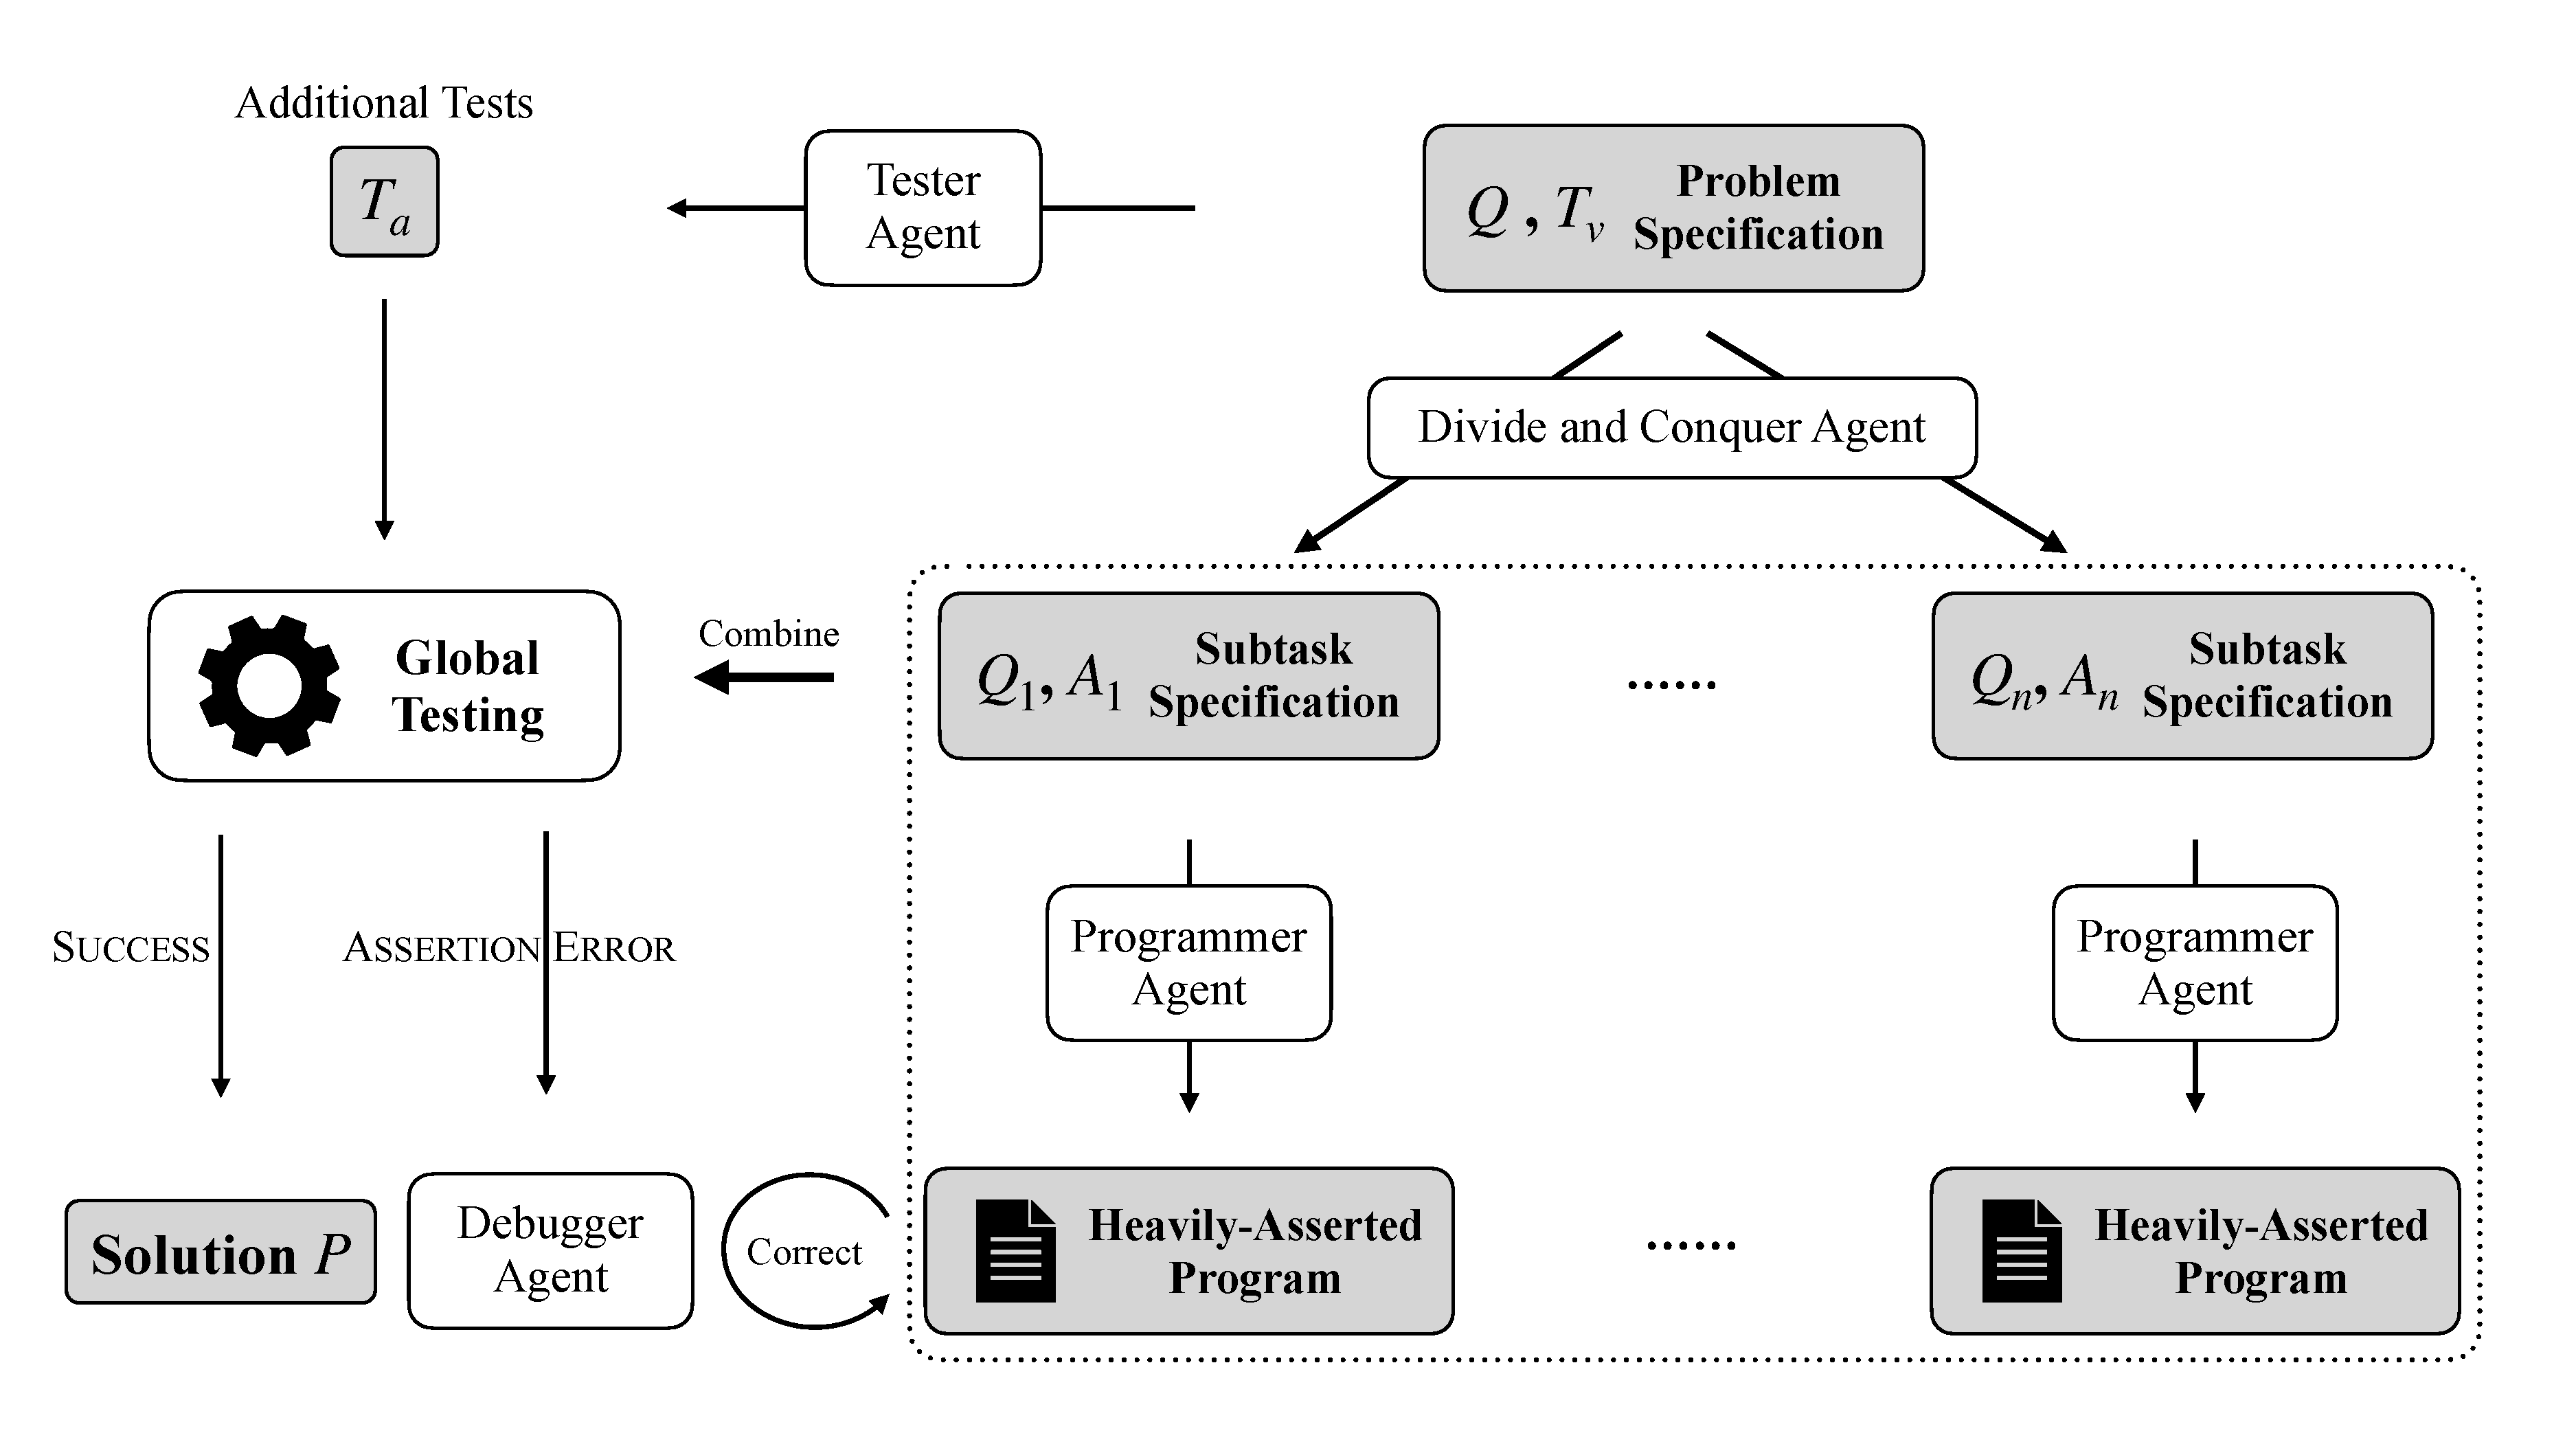
\includegraphics[width=\linewidth]{Architecture.pdf}
    \caption{Overview of the proposed assertion-based debugging framework.}
    \label{fig:overview}
\end{figure*}

Figure~\ref{fig:overview} illustrates an assertion-based debugging framework for large language models (LLMs), which follows a divide-and-conquer approach to problem-solving and debugging. The problem specification will be repeatedly decomposed into smaller subtasks specifications by a divide-and-conquer agent. Each subtask is represented as $(Q_i, A_i)$ where $Q_i$ is the natural language description of the subtask and $A_i$ is a set of assertions that the solution must satisfy. The divide-and-conquer agent will also generate codes to assemble all subprograms into a single unified program. Each subtask will then be assigned to a programmer agent, which generates a heavily-asserted program containing numerous assertions to detect potential errors. These individual programs are later combined into a complete solution using code generated by the divide-and-conquer agent.

While generating the individual programs, the tester agent concurrently generates hundreds of test cases to evaluate the correctness of the program. Once the combined program is generated, the global testing phase evaluates the program using predefined and additional test cases generated by the tester agent. If the program passes all tests, it is accepted as the final solution. Otherwise, if an assertion error is detected, a debugger agent steps in to correct the errors in the program, and the process iterates until a successful solution is reached. The debugger agents are able to navigate the program and identify the root cause of the assertion error, and then decide either to update the assertion or the code. This framework mimics expert debugging techniques by embedding assertions, systematically identifying issues, and refining solutions iteratively.

% It is worth noting that, the debugger agent, the tester agent and the programmer agents in the framework can work \textit{concurrently} without depending on the completion of each other. This parallel processing capability enhances the efficiency and scalability of the framework, enabling rapid debugging and solution generation for complex programming tasks. The framework's modular design allows for easy integration of additional agents or functionalities, making it adaptable to diverse programming scenarios.

\subsection{Prompt Design}

Since the proposed framework requires a large amount of assertions to generated by the programmer agent, the prompt used to guide the LLMs must be carefully designed to produces desired assertions. We must specify exactly what kind of assertions we want the LLMs to generate, and how to incorporate these assertions into the generated code. The prompt design should also consider the balance between the number of assertions and the complexity of the generated code, as an excessive number of assertions may lead to code bloat and performance degradation.

Here we list the important categories of assertions that we aim to specify in the prompt:

\begin{enumerate}
    \item \textbf{Input Assertions} specify the constraints that the input data must satisfy. These assertions are especially useful for checking the correctness of the combination program generated by the divide-and-conquer agent.
    \item \textbf{Output Assertions} specify the expected output of the program. A lot of engineering efforts need to put into those assertions, as they are the most important part of the program. Thus we force the model to generate such assertions, and recommand the model to create helper functions to check the output match the specialization exactly. For example, in a sorting algorithm, an output assertion may specify that the output list must be sorted in ascending order, which may involves a helper function \texttt{isSorted} to ensure that list is completely sorted.
    \item \textbf{Loop Invariants} can potentially help the model to understand the loop structure and the expected behavior of the loop without using information from long-distance context, and thus generate more accurate assertions. This would be more important in the future if we allow the model to interact with program verifiers.
\end{enumerate}



\section{Preliminary Result}

Now we present the preliminary results of our assertion-based debugging framework. We have implemented a simpler version of the architecture in Figure \ref{fig:overview}, with only a single programmer agent and a tester agent, using OpenAI \texttt{gpt-4o} model. We try to evaluate the effectiveness of the framework on HumanEvalPlus~\cite{evalplus}. However, we are not able to finish the evaluation due to the time constraint. We will continue to work on the evaluation and provide the results in the final paper.

Here, we present an example program generated by the programmer agent, as shown in Figure \ref{fig:program}. The program is designed to determine whether any two numbers in a list are closer to each other than a specified threshold. 
The program is heavily-asserted, with assertions to check the input types, the threshold value, and the correctness of the output. The program also includes assertions to verify the correctness of the intermediate results.
While the program is correct and adheres to the given constraints, the test case \pyth{assert has_close_elements([5.0, 5.6, 5.9, 8.0], 0.3) == True}, generated by the tester agent, is incorrect. This is due to standard floating-point semantics, which yield \pyth{5.9 - 5.6 > 0.3}. This highlights the potential advantage of the assertion-based debugging framework, where the programmer agent generates assertions to verify program correctness. These assertions are iteratively refined by the debugger agent, reducing reliance on test cases alone.

\begin{figure*}[t]
\begin{python}
def has_close_elements(numbers: List[float], threshold: float) -> bool:
    """
    Check if in given list of numbers, there are any two numbers closer to each other than
    the given threshold.
    """

    assert isinstance(numbers, list)
    for num in numbers:
        assert isinstance(num, (int, float))
    assert isinstance(threshold, (int, float))
    assert threshold > 0

    if len(numbers) < 2:
        return False

    sorted_numbers = sorted(numbers)

    for i in range(len(sorted_numbers) - 1):
        for j in range(i):
            diff = abs(sorted_numbers[j+1] - sorted_numbers[j])
            assert diff >= threshold
        
        diff = abs(sorted_numbers[i+1] - sorted_numbers[i])
        assert diff >= 0
        if diff < threshold:
            result = True
            assert any(abs(sorted_numbers[k+1] - sorted_numbers[k])\
                < threshold for k in range(len(sorted_numbers)-1))
            return result

    result = False
    for i in range(len(sorted_numbers) - 1):
        diff = abs(sorted_numbers[i+1] - sorted_numbers[i])
        assert diff >= threshold
    assert isinstance(result, bool)
    return result

# Traceback (most recent call last):
#  File "/tmp/testing_python_program.py", line 28, in <module>
#    assert has_close_elements([5.0, 5.6, 5.9, 8.0], 0.3) == True
#           ^^^^^^^^^^^^^^^^^^^^^^^^^^^^^^^^^^^^^^^^^^^^^^^^^^^^^
# AssertionError
\end{python}
\caption{Example of a generated program by the programmer agent.}
\label{fig:program}
\end{figure*}

\section{Project Planning}

We plan to evaluate the proposed assertion-based debugging framework on the HumanEvalPlus and MBPPPlus benchmarks~\cite{evalplus}, which contains a diverse set of programming tasks with natural language descriptions. We will compare the performance of our framework with the state-of-the-art tools mentioned previously. We will evaluate the effectiveness of the framework in detecting and correcting bugs in large language models (LLMs) and generating correct programs for complex programming tasks.

We will try to answer the research questions mentioned in the introduction section based on the evaluation results. To achieve this, we will conduct a series of experiments assessing the debugging success rate, assertion effectiveness, and overall code correctness improvement. Specifically, we will analyze:

\begin{enumerate}
    \item The proportion of errors detected and corrected by the assertion-based approach compared to baseline methods.
    \item The impact of assertion density on the debugging process and whether heavily-asserted programs lead to more effective debugging.
    \item The robustness of the framework across different programming task complexities and error types.
    \item The effect on the evaluation result of different possible designs of the multi-agent framework on the debugging process.
\end{enumerate}

Our evaluation methodology will include both quantitative and qualitative assessments. We will measure standard code evaluation metrics, such as pass rates on benchmark test cases, execution correctness, and debugging efficiency. Additionally, we will conduct an ablation study to determine the contribution of individual components, such as the divide and conquer agent, programmer agent, and debugger agent, to the overall performance.

Finally, based on the findings, we will refine the framework to enhance its effectiveness in real-world debugging scenarios and explore potential improvements, such as integrating adaptive assertion generation and dynamic test case expansion.



% \section*{Accessibility}
% Authors are kindly asked to make their submissions as accessible as possible for everyone including people with disabilities and sensory or neurological differences.
% Tips of how to achieve this and what to pay attention to will be provided on the conference website \url{http://icml.cc/}.

% \section*{Software and Data}

% If a paper is accepted, we strongly encourage the publication of software and data with the
% camera-ready version of the paper whenever appropriate. This can be
% done by including a URL in the camera-ready copy. However, \textbf{do not}
% include URLs that reveal your institution or identity in your
% submission for review. Instead, provide an anonymous URL or upload
% the material as ``Supplementary Material'' into the OpenReview reviewing
% system. Note that reviewers are not required to look at this material
% when writing their review.



% \section*{Acknowledgements}

% \textbf{Do not} include acknowledgements in the initial version of
% the paper submitted for blind review.

% If a paper is accepted, the final camera-ready version can (and
% usually should) include acknowledgements.  Such acknowledgements
% should be placed at the end of the section, in an unnumbered section
% that does not count towards the paper page limit. Typically, this will 
% include thanks to reviewers who gave useful comments, to colleagues 
% who contributed to the ideas, and to funding agencies and corporate 
% sponsors that provided financial support.

% \section*{Impact Statement}

% Authors are \textbf{required} to include a statement of the potential 
% broader impact of their work, including its ethical aspects and future 
% societal consequences. This statement should be in an unnumbered 
% section at the end of the paper (co-located with Acknowledgements -- 
% the two may appear in either order, but both must be before References), 
% and does not count toward the paper page limit. In many cases, where 
% the ethical impacts and expected societal implications are those that 
% are well established when advancing the field of Machine Learning, 
% substantial discussion is not required, and a simple statement such 
% as the following will suffice:

% ``This paper presents work whose goal is to advance the field of 
% Machine Learning. There are many potential societal consequences 
% of our work, none which we feel must be specifically highlighted here.''

% The above statement can be used verbatim in such cases, but we 
% encourage authors to think about whether there is content which does 
% warrant further discussion, as this statement will be apparent if the 
% paper is later flagged for ethics review.

% \nocite{langley00}

\bibliography{example_paper}
\bibliographystyle{icml2025}

\newpage
\appendix
\onecolumn
\section{You \emph{can} have an appendix here.}

You can have as much text here as you want. The main body must be at most $8$ pages long.
For the final version, one more page can be added.
If you want, you can use an appendix like this one.  

The $\mathtt{\backslash onecolumn}$ command above can be kept in place if you prefer a one-column appendix, or can be removed if you prefer a two-column appendix.  Apart from this possible change, the style (font size, spacing, margins, page numbering, etc.) should be kept the same as the main bod.y

\end{document}